\clearpage
\fancyhead[R]{\sffamily\small\color{Muted}一帧的组织与诊断}
\section{场景、绘制命令与渲染线程}

神庙的长廊里有多件共用石材的模型。改动一盏灯时，可以继续使用石柱的网格和纹理。相机看到哪一面、石柱在新灯光下有多亮，则需要重新计算。Redflag 把能长期保存的材质、网格和纹理与本次绘制需要的位置、相机和目标图分开。这样就能单独检查一次材料导入，或一帧中的一次着色。

\begin{figure}[H]\centering
\panelimage{.315\linewidth}{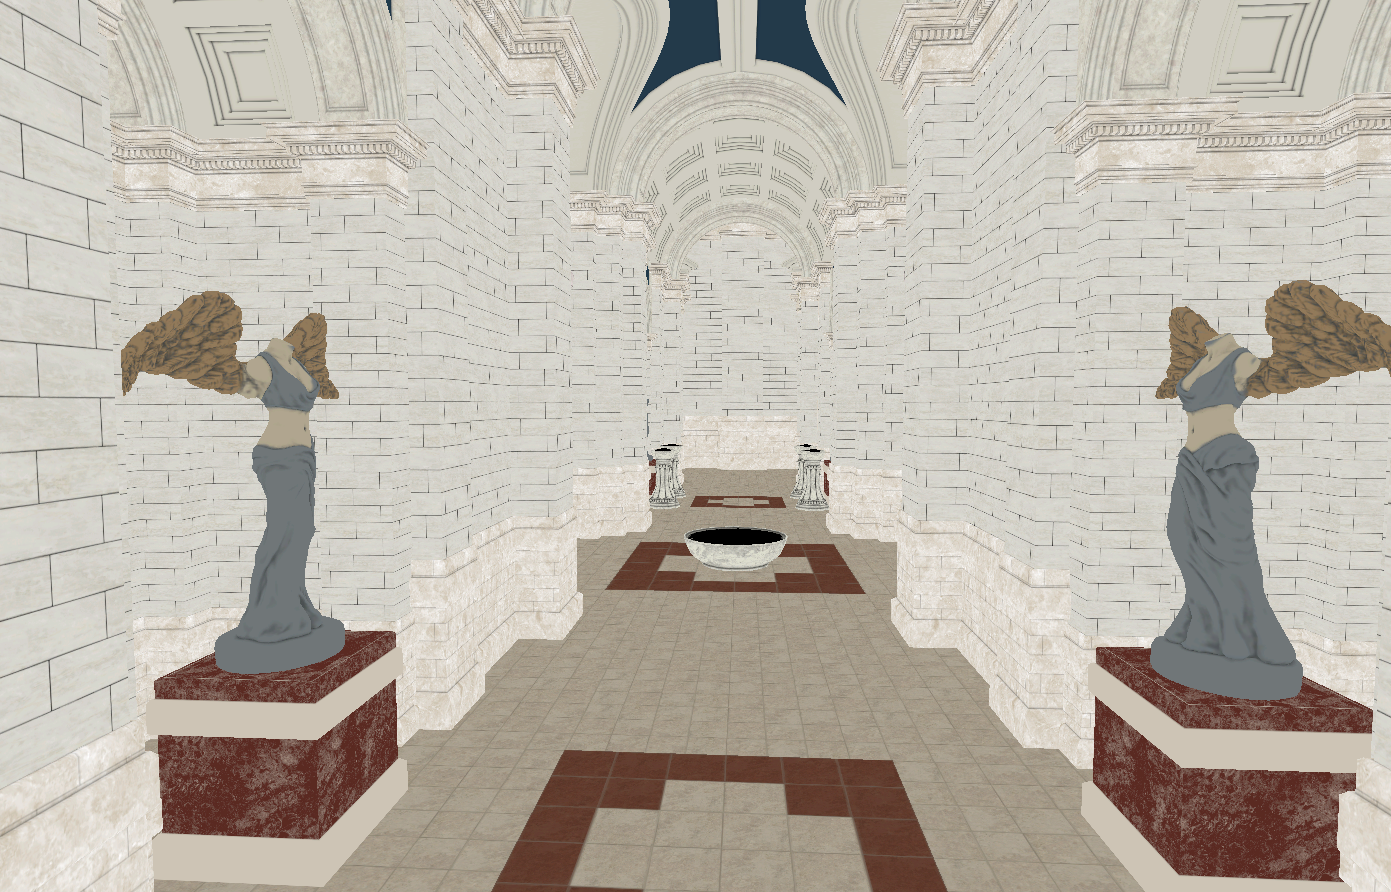
\includegraphics[width=\linewidth]{../../../output/scenes/sun-temple/albedo.png}}{材质底色}
\hfill
\panelimage{.315\linewidth}{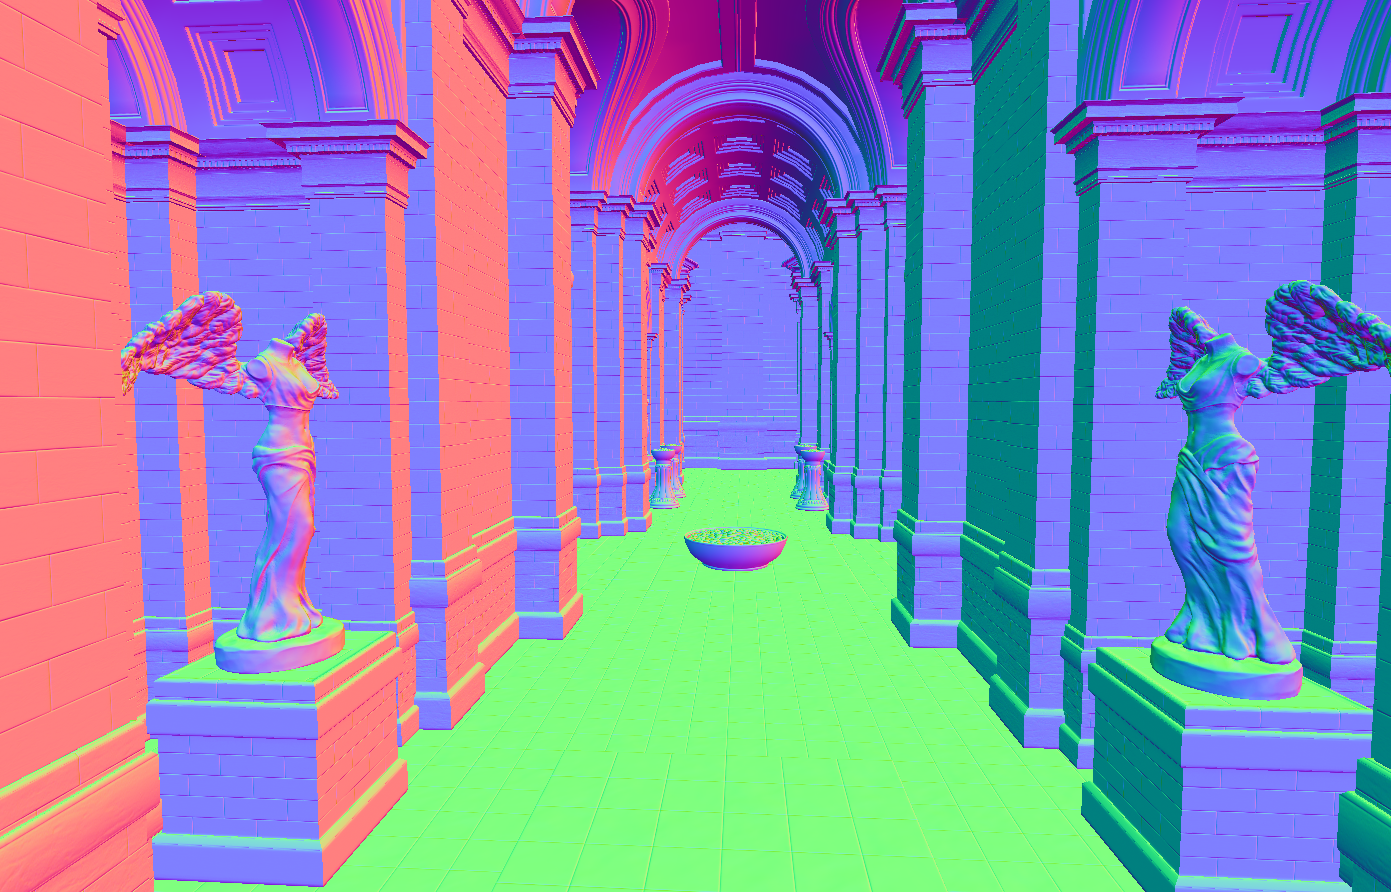
\includegraphics[width=\linewidth]{../../../output/scenes/sun-temple/normal-depth.png}}{表面朝向}
\hfill
\panelimage{.315\linewidth}{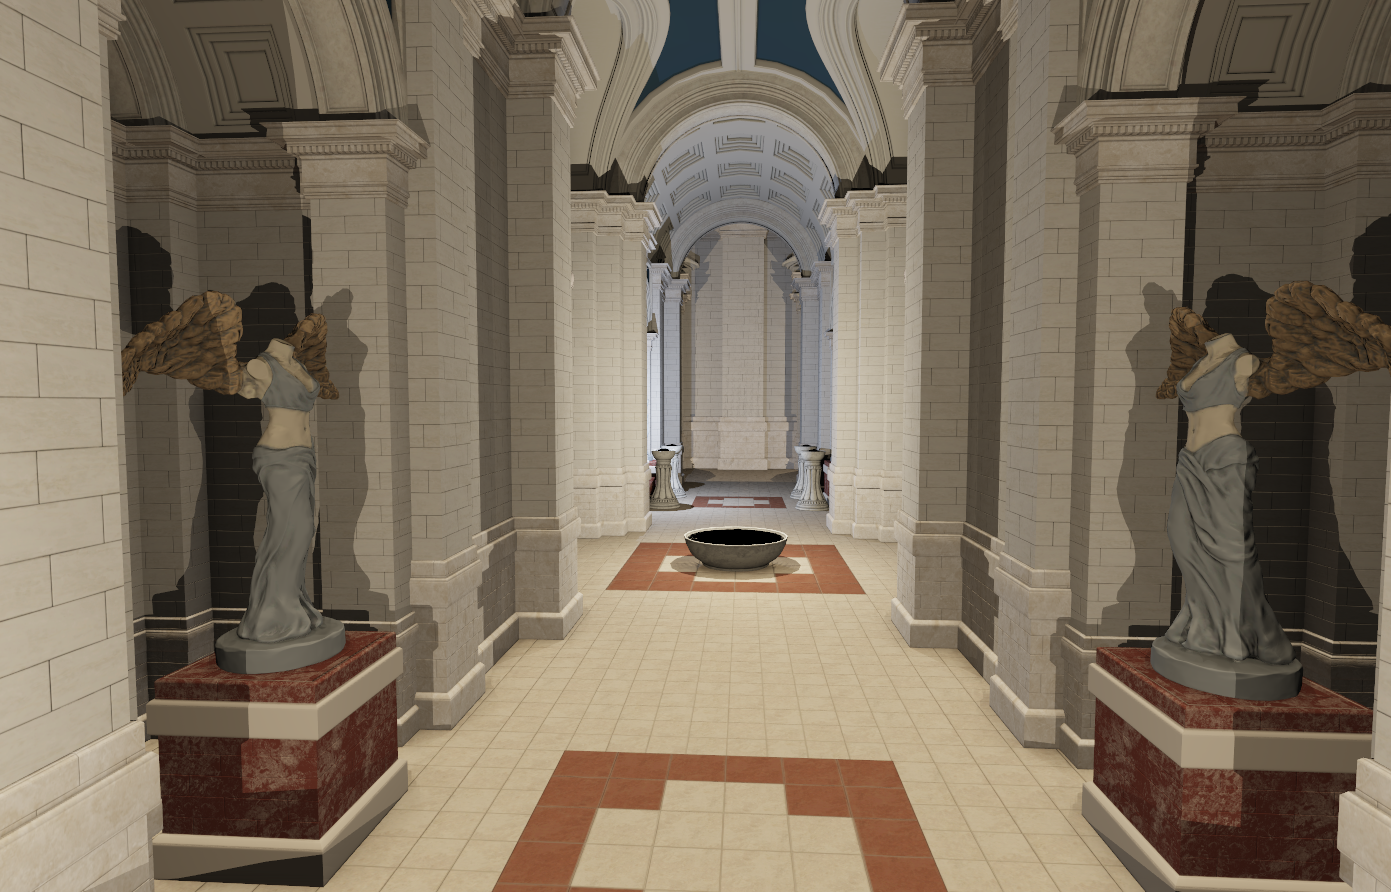
\includegraphics[width=\linewidth]{../../../output/scenes/sun-temple/SunTemple.png}}{编辑器场景颜色}
\caption{Vulkan 编辑器中的同一处神庙。左图能检查纹理是否贴对，中央能检查石柱的轮廓和朝向，右图才把光照加进来。场景由 Epic Games 制作，经 NVIDIA ORCA 发布，CC BY-NC-SA 4.0。}
\end{figure}

\code{Application::Run} 在应用主循环中更新各层，再调用它们的界面绘制。场景和编辑器选择相机、实体、子网格和材质。到 \code{VulkanDraw::DrawIndexed} 时，这些选择已经完成。后端绑定这份网格的顶点和索引，把这次的位置和编号写入命令，再调用 \code{vkCmdDrawIndexed}。这条 draw call 告诉 GPU 从索引中取出哪些三角形。提交命令后，CPU 能继续执行，GPU 在自己的队列上处理绘制。后端按帧保留所用网格和贴图的引用，等这一帧的完成信号（fence）到了，才可以重用该帧的位置、释放这些引用。

UE 的 Game Thread 更新游戏对象，Render Thread 在另一个 CPU 线程上准备渲染。Epic 举的例子是角色组件和它的渲染代理：渲染线程用自己的数据副本，游戏线程可以继续改角色。Redflag 此处沿主循环直接调用后端。若以后把准备命令移到单独线程，先把本帧的变换、材质引用和实体编号固定下来，再交给另一线程。仅把函数放入线程池，会让它读到下一帧甚至已被删除的实体。\source{https://dev.epicgames.com/documentation/en-us/unreal-engine/threaded-rendering-in-unreal-engine}{Epic · Threaded Rendering}

\readings{调用入口见 \path{Redflag/src/Redflag/Core/Application.cpp} 与 \path{Redflag/src/Platform/Vulkan/VulkanDraw.cpp}。神庙的逐事件记录与原始资源许可见 \path{output/scenes/sun-temple/README.md}。}

\clearpage
\section{阶段之间传递的图像}

先看直接光与间接光合成的那一步。直接光是灯直接照到石柱的部分，间接光来自其他表面的反射。GTAO 根据附近的遮挡给出一个零到一的数，放在遮蔽图的透明度通道。下列代码保留直接光，在开关启用时用遮蔽值减弱间接光；同一像素的两部分随后相加。颜色直到显示阶段才转换到屏幕使用的范围。
\begin{lstlisting}
// 只给间接光乘遮蔽。最后加回直接光，写出本像素的线性颜色。
vec3 reflected = hasIndirect != 0 ? indirect[i].rgb : vec3(0);
if (useAO != 0) reflected *= occlusion[i].a;
combined[i] = vec4(direct[i].rgb + reflected, 1);
\end{lstlisting}
{\small\path{RedflagForge/src/Shaders/CombineLight.comp}\quad 计算着色器 \code{main}}\par

\code{LightingPreview::RenderLit} 用普通函数明确排好这几步。选择灯光算法后，先生成直接光和可选的间接光，再合成颜色。SSR 读合成后的场景找倒影。雾要用视线的终点和灯光遮挡，TAA 还要用上一帧留下的结果。关闭一个效果时，把已有的颜色直接传给下一步。选择只看直接光时，算完直接光就可以返回。

UE 的 Render Dependency Graph（RDG）让各阶段先声明自己读写的资源。以同一张合成颜色图为例，图中会有“合成写入，SSR 读取”这条依赖。知道最后一个读者是谁，执行器才有机会回收占用的内存，或在合适的位置安排 GPU 同步。项目当前把顺序和图像保存在 C++ 对象里。固定顺序很容易沿源码检查；将来若多种画法都需要自行判断一张图何时能复用，优先把它们共用的颜色、深度及历史图的读写记录下来，再考虑自动安排。\source{https://dev.epicgames.com/documentation/en-us/unreal-engine/render-dependency-graph-in-unreal-engine}{Epic · Render Dependency Graph}

从一个数据结构就能估显存量级。每个合成像素是一个 \code{vec4}，四个 32 位浮点数占 16 字节。在 $948\times613$ 的面板上，单份颜色数组的数据占 $948\times613\times16=9{,}297{,}984$ 字节，约 8.87 MiB。此前把光照数组换到显卡本地内存，实测 Sponza 的光照更新从 \memoryOld\,ms 变为 \memoryNew\,ms。数组尺寸保持原样，变化在于 GPU 从哪里读它。报告显存节约还需要统计同时存活的所有分配、驱动对齐和峰值；报告帧率则应计完整呈现帧。

\readings{实际输入与输出见 \path{RedflagForge/src/Shaders/CombineLight.comp}，调用与生成数组的位置见 \path{RedflagForge/src/LightingPreview.cpp}。前文「Sponza 的光照数据放在哪里」保留设备、尺寸与逐次计时。}

\clearpage
\section{从一次慢帧定位到具体工作}

64 个不重叠的方块提供了一个可复查的反例。先做深度预写（Pre-Z），GPU 能预先知道每个像素离相机最近的表面。若后面的几何被它挡住，硬件有机会在执行昂贵的片元着色之前就丢弃这些片元，这叫提前深度测试（Early-Z）。不同三角形覆盖同一像素叫重复覆盖（overdraw）。本次方块相互错开，RenderDoc 回放中开关预写，主绘制的片元着色调用都是 43,264 次。打开预写还多了 64 次绘制，GPU 区间中位数从 6.912 增至 9.248 微秒。换成前后重叠的墙面，才值得重新测量它能否减少整帧工作。

同一份深度也能帮忙排错。树叶常画在矩形上，材质用贴图的透明度裁掉空白。曾经主绘制留下孔洞，深度预写却把孔洞也填上，后面的物体便消失了。调试时先看预写结束那一刻的深度，再找叶片着色器用哪张图判断透明。修复让两个阶段使用相同的底色透明度和裁剪阈值。项目用 1,024 个像素逐点比较深度；和主绘制结果相同后，才把问题归到已修复。详见《渲染排错记录》的深度预写实测。

若慢的是合成或光照计算，先定位到具体 dispatch，再改变单一条件。读相邻像素时，临近地址的数据可能已在缓存（cache）里，GPU 便能少从显存取一次。显存带宽是每秒实际传输了多少字节；数组大小乘帧率只能估算数据量。GPU 还把多条线程组成一组来发射指令，这种执行方式叫 SIMT。在 NVIDIA 硬件上，一个 warp 有 32 条线程。如果同组的一些线程沿光线很快遇墙、另一些要走很远，执行不同分支时就可能有一部分线程空等。一次 dispatch 的耗时同时受这些因素影响。

实际排查可以固定灯和相机，先比较相同画面的 CPU 提交与 GPU 时间戳；若 GPU 的某一阶段明显较长，再改变分辨率或每条光线的采样数。当前项目的逐事件和像素证据来自 RenderDoc，区间耗时另由 GPU 查询或独立运行记录。要判断是显存带宽接近上限、缓存命中偏低，还是线程利用率低，可以在 NVIDIA 上针对这个区间再采 Nsight Graphics 的 GPU Trace。PIX 的 GPU Capture 面向 Direct3D 12，可用于对照该后端的事件和计数。此处未采集 Nsight 或 PIX 的硬件计数。

\readings{\path{output/profiling/mesh/replay.json} 记录 Pre-Z 事件，\path{output/profiling/mesh/timing.csv} 保留原始计时。参见 \refitem{https://docs.nvidia.com/nsight-graphics/UserGuide/gpu-trace-overview.html}{Nsight Graphics GPU Trace}、\refitem{https://docs.nvidia.com/cuda/cuda-c-programming-guide/index.html}{NVIDIA 的 SIMT 与 warp 说明}及 \refitem{https://learn.microsoft.com/en-us/windows/pix/gpu-captures/gpu-captures-overview}{Microsoft PIX GPU Capture}。}
